%======================================================================
%===  dtuposter - a class to make posters tha comply with the DTU CI
%
% Written and maintained in 2011-2014 
% by Jorrit Wronski (jowr@mek.dtu.dk)
%
% tex_dtu_aqua_b_uk
%
%==========================================
%===  details and poster setup
\documentclass[
    ,title     = {{Bayesian Additive Regression Trees with Model Trees}}
    ,author    = {{Estevao B. Prado}}
    ,subject   = {{This is the subject of my work}}
%    ,bgcolor   = dtulightgreen
    %,highlight = orange
   ,toplogo   = {{header_poster}}
   %,botlogo   = {{logo.pdf}}
%    ,papersize = {{a0paper}}
%    ,colcount  = {{1column}}
,longtitle
%    ,largecaption
%    ,draft
%    ,nocrops
%    ,english        % language
%    ,fleqn          % equations on the left
]{dtuposter}
%
%
%======================================================================
%===  Continue with packages
\usepackage[T1]{fontenc}        % special characters
%\usepackage[utf8]{inputenc}
%
%\usepackage[ansinew]{inputenc}  % Windows
%\usepackage[applemac]{inputenc} % MacOS
\usepackage[utf8x]{inputenc}    % Unicode, Linux
%
% 
%======================================================================
%=== Font definitions, DTU recommends Arial for posters
\usepackage{cmbright}
\usepackage{arevmath}
\usepackage{amsmath}
\usepackage{biblatex}
\addbibresource{refs.bib}

%\usepackage[scaled]{uarial} %Arial clone, set as default sf font - use "ua1" for direct access
%\usepackage{uarial} %Arial clone, set as default sf font - use "ua1" for direct access
%\usepackage[typeface=default,
%            sanstypeface=urwarial,
%            mathtypeface=arevmath
%           ]{typeface}
\renewcommand{\familydefault}{\sfdefault}
\usepackage{enumitem}
\setlist{nosep,leftmargin=*}
%
% 
%======================================================================
%=== Other useful packages
\usepackage{booktabs}
\usepackage{siunitx}
%
% 
%======================================================================
%=== The actual content starts here
\begin{document}
%
%
%======================================================================
%===  Make header for poster (title and authors)
\begin{dtuposterhead} %
\dtuposterauthor{Estev\~ao B. Prado, Rafael A. Moral, % \textsuperscript{2}, 
 Andrew C. Parnell %\textsuperscript{3}
 }
%\dtuposteraffil{\textsuperscript{1,2,3} Hamilton Institute, Maynooth University, Maynooth, Ireland}
\dtuposteraffil{Hamilton Institute, Maynooth University, Maynooth, Ireland}
\dtuposteraffil*{Corresponding author. Email: \texttt{estevao.prado@mu.ie}}
\end{dtuposterhead}
%
%
%======================================================================
\begin{dtupostercontent}
\section{Introduction}

\begin{itemize}
    \item Bayesian Additive Regression Trees (BART) is a statistical method proposed by \cite{chipman2010bart} that has become popular in recent years due to its competitive performance on regression and classification problems, when compared to other supervised machine learning methods, such as Random Forests (RF) and Gradient Boosting (GB).

     \item In this work, we introduce the algorithm MOTR-BART, which combines Model Trees \cite{quinlan1992learning} with BART to deal with local linearity at node levels. In MOTR-BART, rather than estimating a constant as the predicted value as BART does, for each terminal node a linear predictor is estimated, including only the covariates that have been used as a split in the corresponding tree. With this approach, we aim to capture linear associations between the response and covariates and then improve the final prediction.
\end{itemize}

%======================================================================
%======================================================================
\section{BART}
Introduced by \cite{chipman2010bart}, BART is a tree-based machine learning method that estimates a univariate response by a sum-of-trees as
$$
\begin{aligned}
y_{i} = \sum_{t = 1}^{m} g(\textbf{x}_{i}; T_{t}, M_{t}) + \epsilon_{i}, \mbox{ } \epsilon_{i} \sim \mbox{N}(0, \sigma^{2}),
\end{aligned}
$$
where $g(\textbf{x}_{i}; T_{t}, M_{t})$ is a function that assigns a predicted value $\mu_{t \ell}$ based on the covariates $\textbf{x}_{i}$, $T_{t}$ is the set of splitting rules that defines the $t$-th tree and $M_{t} = (\mu_{t1}, ..., \mu_{t b_{t}})$ is the set of predicted values for all nodes in the tree $t$.

\begin{figure}
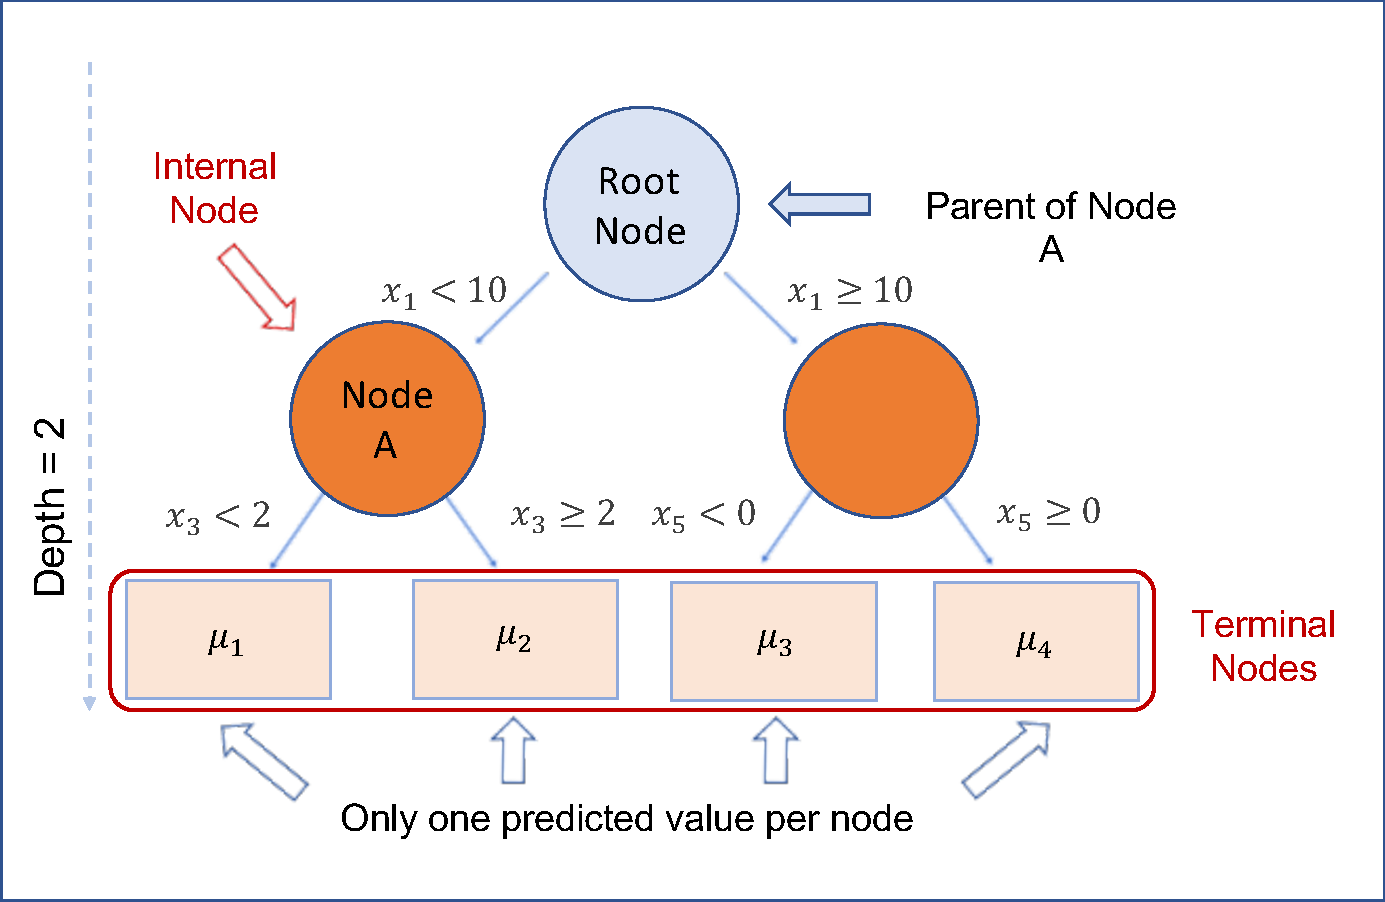
\includegraphics[width=.95\linewidth,origin=c]{Model_trees_plot1.pdf}
\caption{ \hspace{-2.18cm} An example of a single tree generated by BART. In practice, BART generates multiple trees for which the predictions are added together.}
\end{figure}

%======================================================================
%======================================================================

\section{BART with Model Trees}

In MOTR-BART, we consider that the response variable is a sum of trees in the form of
$$\textbf{y} = \sum_{t = 1}^{m} g(\textbf{X}; T_{t}, B_{t}) + \epsilon,$$
where $B_{t}$ is the set of parameters of all linear predictors for the tree $t$. In terms of partial residuals, MOTR-BART can be represented as 
$$
\begin{aligned}
r_{i}|\textbf{x}_{i}, \boldsymbol\beta_{t \ell}, \sigma^{2} & \sim \mbox{N}(\textbf{x}_{i} \boldsymbol\beta_{t \ell}, \sigma^{2}), \\
\end{aligned}
$$
\noindent
where $r_{i} = y_{i} - \sum_{j \neq t}^{m} g(\textbf{x}_{i}; T_{j}, B_{j})$ and $\boldsymbol\beta_{t \ell}$ is the parameter vector associated to the terminal node $\ell$ of the tree $t$. In this sense, all observations $i \in \mathcal{P}_{t \ell}$ will have predicted values based on $\boldsymbol\beta_{t \ell}$ and the values of their covariates $\textbf{X}_{t \ell}$. Thus, each observation $i \in \mathcal{P}_{t \ell}$ may have different predicted values.

\begin{figure}
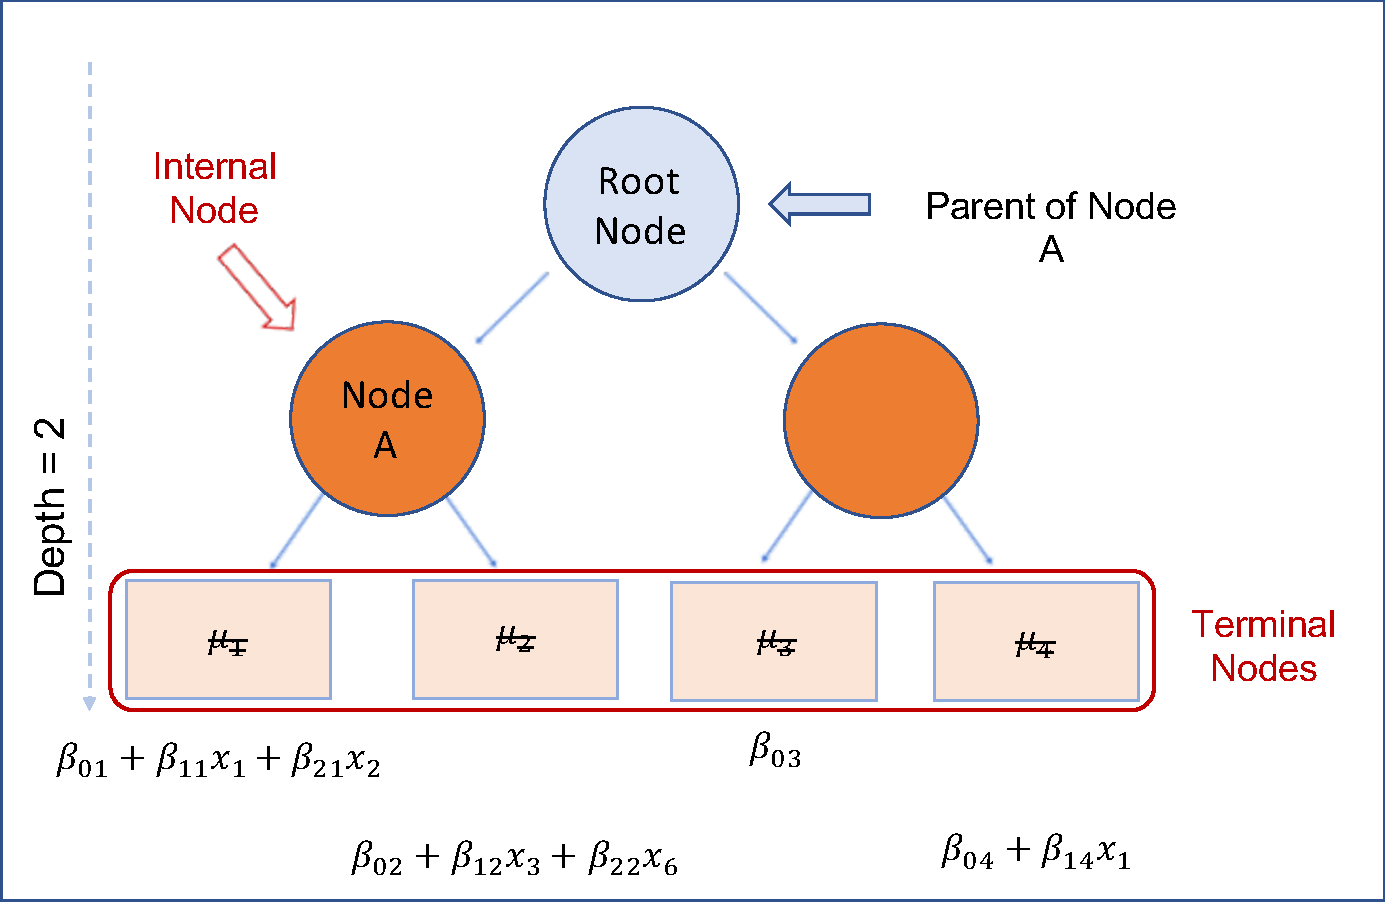
\includegraphics[width=.95\linewidth,origin=c]{Model_trees_plot2.pdf}
\caption{An example of a single tree generated by MOTR-BART.}
\end{figure}

%======================================================================
%======================================================================

\section{Implementation}

MOTR-BART implementation is available in the format of an R package at \url{https://github.com/ebprado/MOTR-BART}.

%======================================================================
%======================================================================

\section{Results for real data}
We compare the predictive performance of MOTR-BART to RF, GB, BART, soft BART, and Local Linear Forests (LLF), in terms of RMSE, on four real data sets. Below, we show the results for two data sets.
\begin{figure}
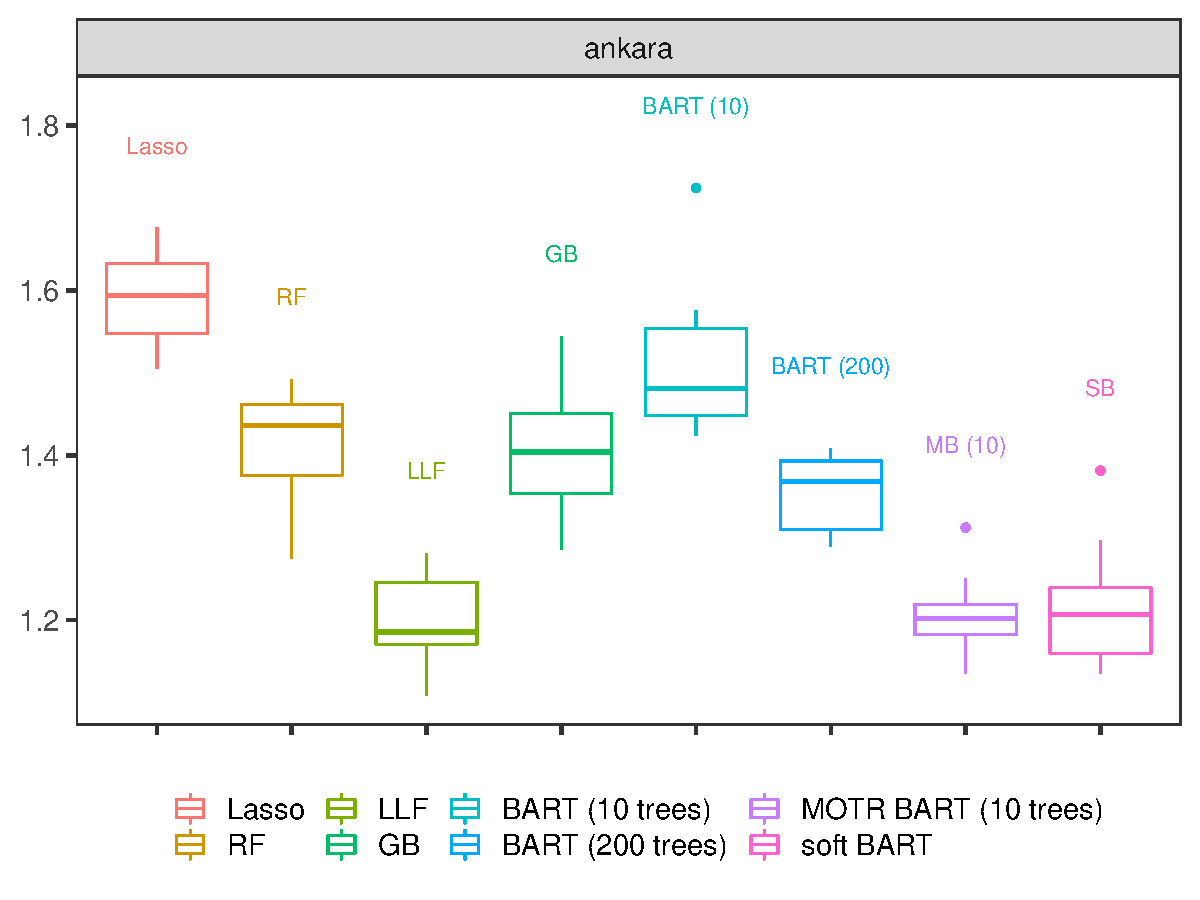
\includegraphics[width=.95\linewidth,origin=c]{ankara.pdf}
\caption{\hspace{-0.799cm} Comparison of RMSE for Ankara data set on 10 different test data.}
\end{figure}

\begin{figure}
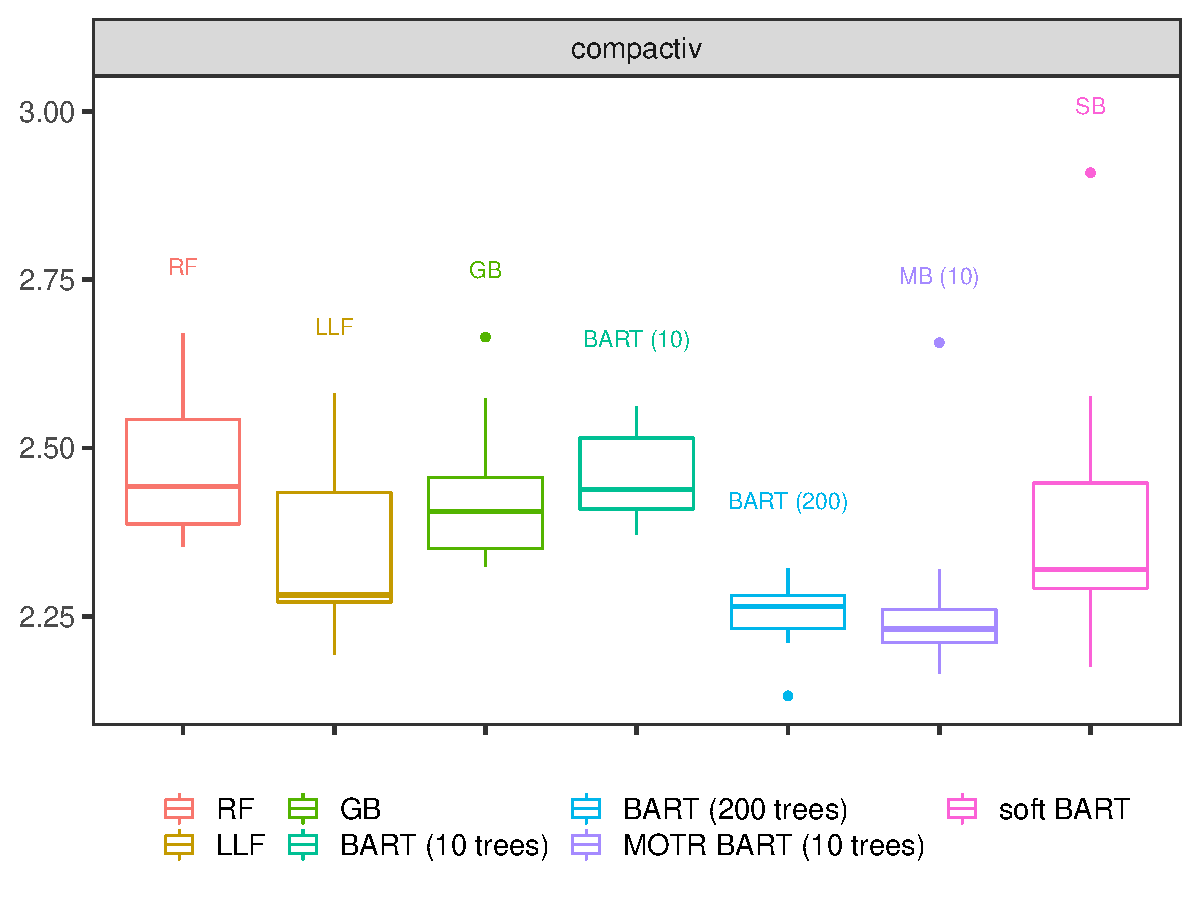
\includegraphics[width=.95\linewidth,origin=c]{compactiv.pdf}
\caption{\hspace{-1.1cm} Comparison of RMSE for Compactiv data set on 10 different test data.}
\end{figure}

\begin{itemize}
    \item MOTR-BART presents the \textbf{best or the second best} results.
    \item It requires \textbf{far fewer} trees to achieve equal or better performance than BART.
\end{itemize}

%======================================================================
%======================================================================

\section{Discussion}

\begin{itemize}
    \item To evaluate variable importance or even to select the covariates in the linear predictors is not straightforward in MOTR-BART.
    \item Splines can be introduced to capture local non-linear behaviour.
\end{itemize}

\printbibliography

\end{dtupostercontent}

\end{document}
